\documentclass[]{article}


\usepackage{amsmath, graphicx, fullpage}

\usepackage{tikz}
\usetikzlibrary{shapes.geometric, arrows}

\tikzstyle{startstop} = [rectangle, rounded corners, minimum width=3cm, minimum height=1cm,text centered, text width=3cm, draw=black, fill=red!30]
\tikzstyle{io} = [trapezium, trapezium left angle=70, trapezium right angle=110, minimum width=3cm, minimum height=1cm, text centered, text width=2cm, draw=black, fill=blue!30]
\tikzstyle{process} = [rectangle, minimum width=3cm, minimum height=1cm, text centered, text width=3cm, draw=black, fill=orange!30]
\tikzstyle{decision} = [rectangle, minimum width=3cm, minimum height=1cm, text centered, text width=3cm, draw=black, fill=green!30]
\tikzstyle{arrow} = [thick,->,>=stealth]

\begin{document}


\title{DynoGrid\\{\Large Dynamically Load-Balanced PIC Code with an Adaptive Grid}}

\author{Scott \textsc{Luedtke}, Max \textsc{Porter}, Joel \textsc{Iventosch}, Mark \textsc{Sholte}}

\maketitle

\section{Introduction}

Particle in Cell (PIC) codes are commonly used to simulate plasma physics.  Existing codes, such as EPOCH~\cite{epoch}, allow physicists to simulate many experiments, including laser experiments.  Larger problems, such as 3D simulations of high-intensity laser experiments like those performed on the Texas Petawatt Laser (TPW), are too computationally expensive to run on modern supercomputers.  One way to bring these problems down to size is to adaptively change the grid size.  Simulations can require a very high resolution at certain sites (for example, where a laser hits a target), and orders of magnitude coarser resolution throughout the rest of the simulation.

We have developed a 3D PIC code with a standard Boris particle pusher \cite{bird}, added an adaptive grid, implemented data passing routines among nodes, and load balanced the work based on the changing grid.  Our code is not physically accurate, ommiting a field solver and ignoring many physically relevant effects, but we believe it is an accurate representation of a production code in performance characteristics and expect our load balancing to behave similarly on a production code.


\section{Code Description}
PIC codes are commonly used in computational physics.  A PIC code typically consists of an array of grid points that define electromagnetic field values, and particles that move continuously throughout the grid.  We created a fairly simple 3D laser-plasma code with externally defined fields (the laser), and physical effects such as particle collision and photon pair production omitted.  We did however add an adaptive grid which makes load balancing more complex.

\subsection{Particle Pusher}
Particle-in-cell (PIC) codes used to simulate laser-plasma interactions commonly use the Boris pusher \cite{bird}, a second order accurate pusher for charged particles in electromagnetic fields.  The pusher is outlined in Fig.~\ref{fig:boris}.  Essentially, the particle is advanced a half time-step, the momentum is updated with $\vec{E}$ and rotated with $\vec{B}$, and the particle is moved a final half time-step.  With a properly set time step, a particle will never move more than one cell.


\begin{figure}[htbp]
\centering
\caption{Schematic of the Boris pusher.  The sub-cycling and current and density calculations were not implemented.}
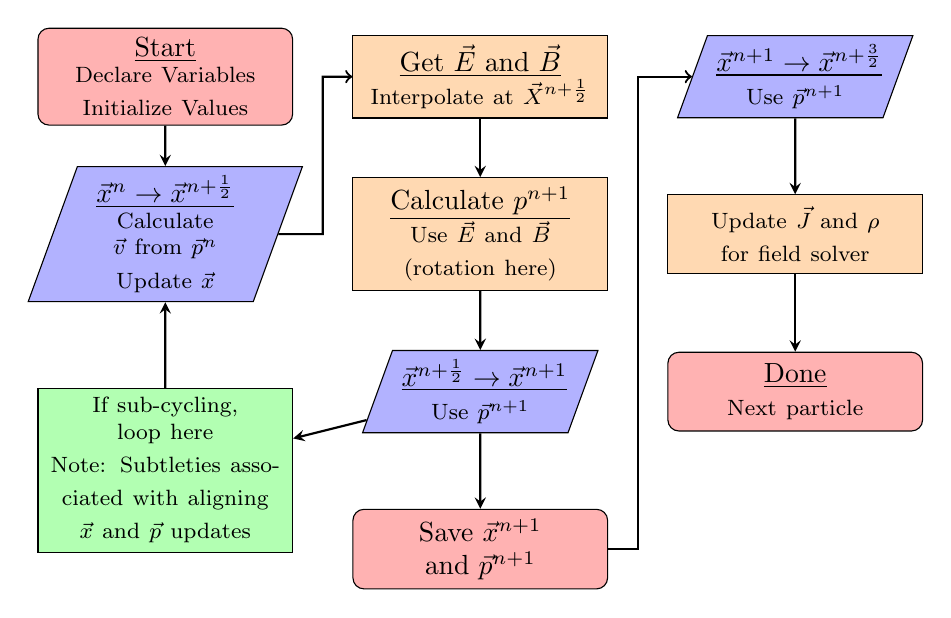
\begin{tikzpicture}[node distance=2cm]

\node (start) [startstop] {\underline{Start}\\{\footnotesize Declare Variables\\Initialize Values}};

\node(pos1)[io, below of=start]{\underline{$\vec{x}^n \rightarrow \vec{x}^{n+\frac{1}{2}}$}\\{\footnotesize Calculate $\vec{v}$ from $\vec{p}^n$\\Update $\vec{x}$}}; 

\draw[arrow](start) -- (pos1);

\node(EB)[process, right of=start, xshift=2cm]{\underline{Get $\vec{E}$ and $\vec{B}$}\\{\footnotesize Interpolate at $\vec{X}^{n+\frac{1}{2}}$}};

\draw[thick,->] (pos1) -- +(2,0) |- (EB);

\node(pn1)[process, below of=EB]{\underline{Calculate $p^{n+1}$}\\{\footnotesize Use $\vec{E}$ and $\vec{B}$ (rotation here)}};

\draw[arrow](EB) -- (pn1);

\node(pos2)[io, below of=pn1]{\underline{$\vec{x}^{n+\frac{1}{2}} \rightarrow \vec{x}^{n+1}$}\\{\footnotesize Use $\vec{p}^{n+1}$}};

\draw[arrow](pn1) -- (pos2);

\node(save)[startstop, below of=pos2]{Save $\vec{x}^{n+1}$ and $\vec{p}^{n+1}$};

\draw[arrow](pos2) -- (save);

\node(pos3)[io, right of=EB, xshift=2cm]{\underline{$\vec{x}^{n+1} \rightarrow \vec{x}^{n+\frac{3}{2}}$}\\{\footnotesize Use $\vec{p}^{n+1}$}};

\draw[thick,->] (save) -- +(2,0) |- (pos3);

\node(cur)[process, below of=pos3]{{\footnotesize Update $\vec{J}$ and $\rho$ for field solver}};

\draw[arrow](pos3) -- (cur);

\node(end)[startstop, below of=cur]{\underline{Done}\\{\footnotesize Next particle}};

\draw[arrow](cur) -- (end);

\node(sub)[decision, left of =pos2, xshift=-2cm, yshift=-1cm]{{\footnotesize If sub-cycling, loop here\\Note: Subtleties associated with aligning $\vec{x}$ and $\vec{p}$ updates}};

\draw[arrow](pos2) -- (sub);
\draw[arrow](sub) -- (pos1);

\end{tikzpicture}
\label{fig:boris}
\end{figure}

Our pusher follows the implementation in EPOCH \cite{epoch}, but with some modifications.  We use our own linear interpolation method (for simplicity), and omit the steps necessary for the field solver, which we did not implement.  We have different logic for finding the field points nearest a particle, and recursive logic to find the finest grid cell a particle is in.  In addition, we have a particle list for each base cell, and implemented logic to pass particles between lists (this makes the load balancing easier).

\subsection{Particle Lists}

\subsection{Grid Trees}
In order to simulate electromagnetic fields, the area of the simulation must be discretized, with each point on its grid holding 3D values for the electric and magnetic fields $\vec{E}$ and $\vec{B}$. Since we are implementing an adaptive grid, we chose to represent our grid cells with a data type called a tree. A tree holds various information only at the coarsest cell size, such as the particles located in that cell, the cell position relative to the entire grid over all processors (a.k.a. its global position), and the ID of the processor that owns it. It also holds a pointer to a tree node, which contains the eight corner grid points (their $\vec{E}$ and $\vec{B}$ fields) and 8 recursive pointers to (potential) tree node children. This allows for an efficient adaptive grid by separating data which is only needed at the coarsest grid level from data which needs to recurse, and therefore removing any unnecessarily repeated information.

As an additional note, it happens that treating each grid cell as an object (rather than, say, having a global array of grid points) leads to the possibility of repeated grid points since each point is "owned" by eight different cells. However we took care to prevent these repeats by having each cell be in charge of a single grid point, and simply point to the grid points of seven other neighbor cells. In order to not miss any grid points in this fashion, we then added a layer of "ghost cells" that each contribute one grid point without otherwise affecting the simulation.

It may also be helpful to explain the purpose of having each grid cell keep track of its owner. With our previously described particle pusher, it is necessary for each processor to keep a copy of every neighboring cell which is adjacent (or diagonal) to a cell it owns, so that it can accurately simulate its particles moving into those cells (and therefore being transferred to other processors). In order to distinguish between these neighbor cells and its own cells, every cell simply remembers who its real owner is.

\subsection{Grid Refinement}
Grid refinement is how we execute the idea of an adaptive grid. An adaptive grid is a grid which starts at a "base" grid spacing which is relatively low, then dynamically becomes finer only where deemed necessary. The condition we use to determine how refined a given grid cell needs to be is the variation of the electric and magnetic fields across that cell. If the variation is large, we conclude that the cell does not have enough resolution to properly represent that cell and therefore we choose to refine it. If a cell has been refined, but the variation across its cell (and the cells of its children) becomes relatively small, it concludes that the extra resolution is no longer necessary and chooses to coarsen. Refinement can also be done recursively on the generated children, and therefore, up to physical limits, refinement can occur as many times as necessary.

Since our tree data type is recursive, our grid refinement algorithm is also, of course, recursive. Our algorithm consists chiefly of two functions: refine() and coarsen(). As the names would suggest, refine() causes a tree node (see "Grid Trees") to generate 8 children, each half of its size in each dimension, and coarsen() causes a tree node to destroy its children, establishing itself as the most refined cell size at that location. At each time step, every grid cell is asked three questions: Does it need to coarsen? Does it need to refine? And do its children need to coarsen or refine? Since this acts recursively at each time step, any amount of refinement or coarsening can happen in a single step, so the refinement level of the grid can never fall behind the current demand.


\section{Parallelization}

\subsection{Particle List Passer}
Particles move throughout the simulation volume and often end up in a different cell at the end of any given time step.  Since different cells can be on different processors, all processors must stop at the end of every time step to pass particles and reconcile their differences with neighbors.  To facilitate this, each base grid cell keeps a list of the particles in it and a separate list of the particles that hove moved into it.  All of the particles that need to be passed are thus in the second list of the ghost cells and there is no need to traverse a list of all particles to find those that need to be passed.  This is implemented in three steps in functions in \texttt{push.c}, \texttt{mpicomm.c}, and \texttt{mpi\_dyno.c}.

Before the communication, each processor assembles a list of its neighbors by checking the owner of each of its ghost cells.  The neighbor relationship is one-to-one, i.e., if A is B's neighbor, B is A's neighbor.  Thus each processor can communicate directly with only the processors it needs to.

First, each processor communicates to each neighbor how many particle lists it will pass, so the neighbors know how many to expect.  This is followed by an \texttt{MPI\_WaitAll} command to ensure synchronization.  Next, the neighbors communicate the size of each list to be sent, followed by another \texttt{MPI\_WaitAll}.

In the third step, the particles are themselves passed.  First, the singly-linked lists of particles are packed in to buffers that are continuous arrays of particles.  These buffers are then sent.  Memory for the receive is allocated based on the previous two communications and the receive is executed, followed by a final \texttt{MPI\_WaitAll}.  Finally, the particles are unpacked into their respective lists.

\subsection{Cell Passer}
During load balancing (explained in the next section) it is necessary to pass cells between processors in order to equilibrate the amount of work required of each processor. This is carried out with the cell passer. The cell passer executes \texttt{MPI\_Isend} and \texttt{MPI\_Irecv} with each of its neighbors along the axis of load balancing, although only up to one of these sends will be non-empty. Since we have chosen the y-axis to be our single axis of load balancing, only processors directly above or below each other trade cells. 

The process of trading cells goes as follows: first the lists to be sent to neighbors are compressed to a convenient, simplified form to minimize the message size. Since each cell actually contains both a cell (grid points plus a global spatial location) and a list of particles, these elements are compressed individually and sent sequentially. After all messages are sent, the cells which are being given away are removed from the local grid. Then all receives are called and waited for. Upon completion, the received data is uncompressed and restored to full cell form, and one cell at a time is added to the grid based on its global spatial position. Care is taken to update the local grid's size and, as may occasionally be necessary, check whether the new cells stray out of bounds of the previously initialized grid, and if so, to re-initialize the grid so that it is centered around the new dimensions with ample padding to avoid another re-initialization in the near future. Finally we ensure that all sends have finished (which they surely have) and exit the cell passer.

\subsection{Load Balancer}


\section{Theoretical Performance}
For sequential performance, performance should depend on the number of particles and grid points in the simulation.  Essentially, computation time should be 
\begin{equation}
\mathcal{O}(N + M),
\end{equation}
where $N$ is the number of particles and $M$ is the number of grid points.  Since we are using an adaptive grid, $M$ is not constant, however, we will treat it as a constant here.  I (Scott) expect that full, physics-accurate simulations will refine in one area and simultaneously coarsen in another, keeping the total number (but not the processor distribution) of grid points generally constant.  This is especially true for our test problem.

\section{Performance Results}

\section{Discussion}
Despite all that we accomplished in this project, the size of what we aimed to achieve ended up greater than we could manage. Most notably, the logic for load balancing in all three dimensions proved too convoluted to figure out and implement in the time available, so we opted for a (still challenging) one-dimensional balancer instead. The choice of going one-dimensional rather than, say, two-dimensional, is that a large jump in complexity occurs once the faces of processors no longer line up on a one-to-one basis. For instance, it can quickly become the case that each processor is facing two or more processors in each direction, so that during load balancing processor A needs to negotiate with B and C, but the decisions of B are also dependent on D and E, which are also each dependent on F and G and H and J respectively, and so on. It would take significantly longer to solve these decisions of exponential complexity, so we restricted to the more deterministic case in which each processor always has only one neighbor in each direction. There still exist significant challenges here, such as ensuring the propagation of excess loads across the grid when one whole side of the grid has heavier loads than the other. We took care to address this and other concerns to make our one-dimensional load balancer as effective as possible.

\section{Whodunit}
Scott Luedtke was primarily responsible for the particle pusher and load balancer.  Since this project is closely related to Scott's research, he oversaw the physics and provided general guidance for what the code should accomplish.

Max Porter was most frequently responsible for grid-related functions. He wrote the grid (and particle) initializations, the laser, and much of the (rather complicated) grid cell passer. He also worked out bitwise logic on several occasions.

Joel Iventosch wrote the output and visualization routines and helped with MPI passing.  He also helped with the grid refinement.

Mark Sholte wrote much of the list functions and tree structure.  He also managed any git repository issues that arose and proved a masterful debugger.

\section{Conclusions}
























{\def\section*#1{}
\begin{thebibliography}{1}
%\footnotesize
\setlength{\itemsep}{0pt}
\bibitem{epoch}The EPOCH code was developed as part of the UK EPSRC funded projects EP/G054940/1
\bibitem{bird}Birdsall, C.K. and Langdon, A.B.  (1985). \textit{Plasma Physics via Computer Simulation}. McGraw-Hill.
%\bibitem{three}Po Kin Leung et al. 2011 Astrophysical Journal, 737 21.
%\bibitem{four}Feryal Özel et al. 2000 Astrophysical Journal, 541 234.
%\bibitem{rotation}Arefiev, Alexey V., et al. ``Temporal resolution criterion for correctly simulating relativistic electron motion in a high-intensity laser field."  Phys. Plasmas 22, 013103 (2015)

\end{thebibliography}
}




\end{document}